\documentclass{IEEEtran}

\usepackage{mathtools}
\usepackage{graphicx}
\usepackage{subfig}
\usepackage{verbatim}
\usepackage{algpseudocode}
\usepackage{natbib}
\usepackage{url}
\usepackage{listings}
\usepackage[spanish]{babel}
\usepackage[utf8x]{inputenc}
\usepackage{float}
\setcounter{MaxMatrixCols}{16}

\begin{document}

\title{Informe Tarea No 2}
\date {Abril de 2013}
\author{\IEEEauthorblockN{Tatiana Lopez Guevara \\}
\IEEEauthorblockA{Universidad Tecnológica de Pereira\\
zepolitat@utp.edu.co }}
\maketitle


\begin{abstract}
El presente documento explica los resultados obtenidos al remover
las distorciones proyectiva y afín haciendo uso de las
estructuras propias de la imágen, a diferencia del trabajo 1 en
donde se daban explícitamente la correspondencia entre la imágen original
y la distorsionada para 4 pares de puntos.
\end{abstract}

\begin{IEEEkeywords}
Computer Vision
\end{IEEEkeywords}

\section{Rectificación Afín}

A diferencia de una transformación proyectiva, en una transformación afín
las líneas paralelas permanecen paralelas, es decir,
los puntos ideales que forman la línea al infinito $L_{\infty}$
permanecen en el infinito. Resulta conveniente entonces aprovechar esta característica
invariante para identificar una matrix de transformación $H$ que vuelva a enviar
la línea de desvanecimiento nuevamente al infinito, removiendo así la perspectiva 
\cite{hartley2000multiple}.

La primera parte del trabajo consistió en identificar dentro de la imágen 2 conjuntos de 
pares de líneas $(l_1, l_2)$ y $(m_1, m_2)$ que se sabe que son paralelas en el mundo real.
Luego, se obtuvo la línea de desvanecimiento $vl$ mediante (\ref{eq:vl}).

\begin{align}
P &= l_1 \times l_2 \nonumber \\
Q &= m_1 \times m_2 \nonumber \\
vl &= P \times Q
\label{eq:vl}
\end{align} 

En la figura \ref{fig:iImg} se muestra la imágen con la distorción proyectiva.

\begin{figure}[H]
\caption{Imágen con distorción proyectiva}
\centering
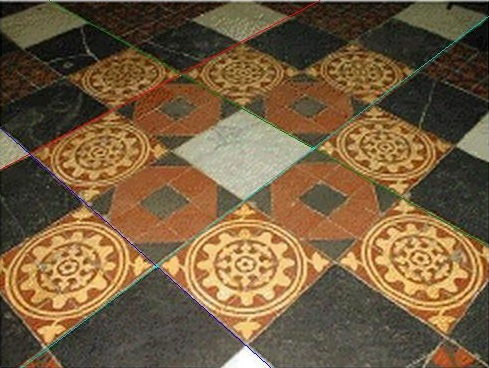
\includegraphics[width=7cm,natwidth=489,natheight=368]{imgs/i1Img.jpg}
\label{fig:iImg}
\end{figure} 

La matriz H se obtiene entonces mediante
\begin{equation}
H = 
\begin{pmatrix}
1 & 0 & 0 \\
0 & 1 & 0 \\
vl_1 & vl_2 & vl_3\\
\end{pmatrix}
\label{eq:h}
\end{equation} 

Una vez conocida la matriz H, lo primero que se hizo 
fue hallar el tamaño de la imágen 
final. Para esto se aplicó la homografía inversa sobre
las esquinas de la imágen cargada empleando (\ref{eq:x}).

\begin{equation}
x=H^{-1} x^{'}
\label{eq:x}
\end{equation} 

Teniendo entonces el tamaño de la imágen, se procedió a 
encontrar para cada punto $(x,y)$ de la imágen
final, su equivalente $(x^{'},y^{'})$. Cabe notar
que a pesar de que (\ref{eq:xp}) hace referencia a la transformación 
de un solo punto, en el desarrollo se usó la representación matricial
en donde $x$ es el conjunto de puntos de la forma 
$[x_1 y_1 1; x_2 y_2 1; .. x_N y_N 1]'$ y por lo tanto $x'$ contiene
todos los puntos transformados de $x$;

\begin{equation}
x^{'}=H x
\label{eq:xp}
\end{equation} 

El inconveniente al hallar los puntos $(x^{'},y^{'})$ que se obtienen de 
(\ref{eq:xp}), es que éstos pueden no ser enteros y por lo tanto
se debió aplicar una técnica de interpolación (ver sección \ref{sc:interp}).

Finalmente, al remover la perspectiva y aplicar la interpolación bilineal sobre
la figura \ref{fig:iImg} se obtubo la figura \ref{fig:faImg}.

\begin{figure}%[H]
\caption{Imágen rectificada hasta afinidad. (a) Resultado obtenido
en este trabajo. (b) Resultado obtenido con el toolbox de Matlab}
\centering
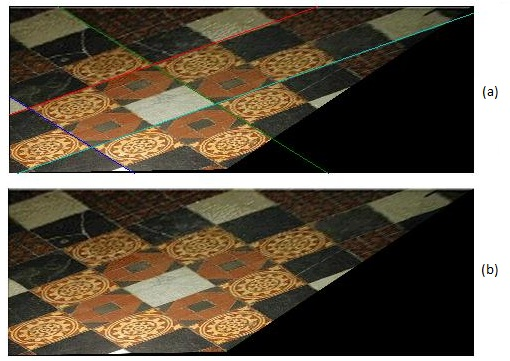
\includegraphics[width=7cm,natwidth=510,natheight=361]{imgs/cvA.jpg}
\label{fig:faImg}
\end{figure} 

\section{Rectificación Métrica}

La segunda parte del proyecto consistió en remover la transformación
afín hasta una similaridad. Para esto se toma ventaja de la cónica $C^*_{\infty}$ 
formada por los puntos circulares $I=(1,i,0)^T$ y $J=(1,-i,0)^T$. 
Esta cónica es invariante ante las trasnformaciones similares 
(\ref{eq:cHs}) y puede ser empleada para medir ángulos 
euclidianos en una proyectividad mediante (\ref{eq:cAng}) 
ya que dicha expresión es invariante ante transformaciones proyectivas \cite{hartley2000multiple}.

\begin{equation}
C^*_{\infty}\vphantom{}'=H_s C^*_{\infty} H_s^T = C^*_{\infty}
\label{eq:cHs}
\end{equation} 

\begin{equation}
\cos\theta = \frac{l^T C^*_{\infty} m}{\sqrt{(l^T C^*_{\infty} l)(m^T C^*_{\infty} m)}}
\label{eq:cAng}
\end{equation} 

Esta última propiedad (\ref{eq:cAng}) permite identificar que para un par de líneas
ortogonales el $\cos 90$ es 0 y por lo tanto:

\begin{equation}
l^T c^*_{\infty} m = 0
\label{eq:cOrt}
\end{equation}

Dados 2 conjuntos de pares de líneas ortogonales y gracias a la 
ecuación (\ref{eq:cOrt}), se puede encontrar $C^*_{\infty}$, o más 
específicamente la matriz $K$ 
resolviendo (\ref{eq:s}) 

\begin{equation}
\begin{pmatrix}
l'_1 & m'_1, l'_1 m'_2 + l'_2 m'_1 \\ 
n'_1 & p'_1, n'_1 p'_2 + n'_2 p'_1 \\
\end{pmatrix}
\begin{pmatrix}
s_{11} \\ s_{12}
\end{pmatrix}
= 
-
\begin{pmatrix}
l'_2 m'_2 \\ n'_2 p'_2
\end{pmatrix}
\label{eq:s}
\end{equation} 

Donde

\begin{equation}
S=
\begin{pmatrix}
s_{11} & s_{12} \\
s_{12} & s_{22} \\
\end{pmatrix}
=
\begin{pmatrix}
K K^T & \vec{0} \\
\vec{0}^T & 0 \\
\end{pmatrix}
\label{eq:sA}
\end{equation} 

Es decir que encontrando $S$ y aplicando la descomposición de Cholesky,
se puede obtener la matriz $K$ que define a la matriz $H_A$ y que remueve
la afinidad.

\begin{equation}
H_A=
\begin{pmatrix}
K & \vec{0} \\
\vec{0}^T & 1 \\
\end{pmatrix}
\label{eq:ha}
\end{equation} 

De forma similar a la parte 1, se realizó el cálculo de la matrix de 
transformación $H$ a partir de los 8 puntos dados. Luego, ésta se usó
para aplicar la distorción proyetiva sobre cada punto de la imágen planar 
mediante (\ref{eq:xp}) .
El resultado obtenido se puede ver en la figura \ref{fig:fsImg}.

\begin{figure}[H]
\caption{Imágen rectificada hasta similaridad. (a) Resultado obtenido
en este trabajo. (b) Resultado obtenido con el toolbox de Matlab}
\centering
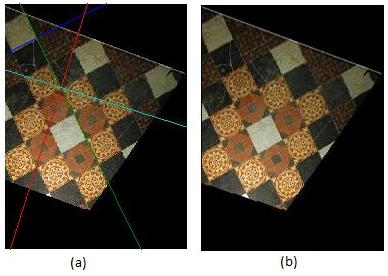
\includegraphics[width=7cm,natwidth=388,natheight=276]{imgs/cvM.jpg}
\label{fig:fsImg}
\end{figure} 

En las figuras \ref{fig:t1I} \ref{fig:t1A} y \ref{fig:t1S} se pueden ver los resultados al
aplicar las 2 partes sobre una fotografía de un cuadro.

\begin{figure}
\centering
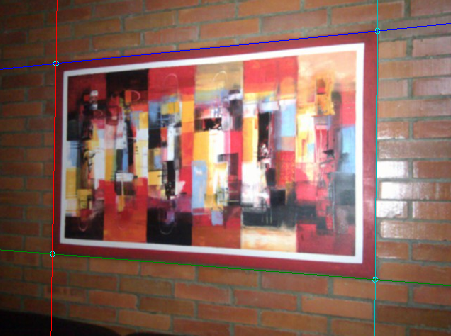
\includegraphics[width=5cm,natwidth=451,natheight=336]{imgs/t1I.png}
\caption{Imágen original.}
\label{fig:t1I}
\end{figure}
\begin{figure}
\centering
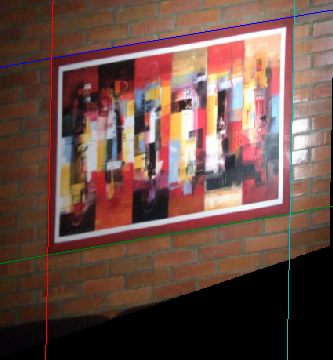
\includegraphics[width=5cm,natwidth=333,natheight=360]{imgs/t1A.png}
\caption{Imágen con corrección proyectiva hasta afinidad.}
\label{fig:t1A}
\end{figure}
\begin{figure}
\centering
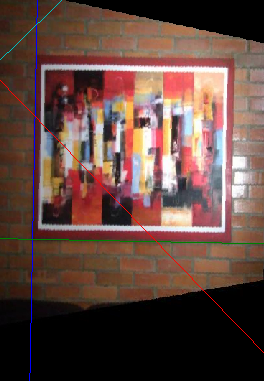
\includegraphics[width=5cm,natwidth=264,natheight=381]{imgs/t1S.png}
\caption{Imágen con corrección afín hasta similaridad.}
\label{fig:t1S}
\end{figure}

\section{Métodos de Interpolación}
\label{sc:interp}
A diferencia de los métodos de interpolación Nearest Neighbor (1 pixel más cercano) e interpolación bilinear (2x2 pixeles más cercanos), la interpolación bicúbica toma en cuenta los 4x4 pixeles más cercanos, dando mayor peso en el cálculo a los que se encuetran más cerca.

Esta técnica consiste en aproximar un valor mediante un polinomio de tercer
grado (\ref{eq:bicubic}).

\begin{equation}
p(x,y) = \sum_{i=0}^{3} \sum_{j=0}^{3} a_{ij} x^i y^j
\label{eq:bicubic}
\end{equation} 

Como se describe en \cite{BicubicWiki}, el problema consiste en identificar
los 16 coeficientes $a_{ij}$ (a partir de los 16 puntos conocidos)
del sistema descrito por (\ref{eq:a}).

\begin{equation}
\vec{\alpha} = A^{-1} \vec{P}
\label{eq:a}
\end{equation} 

Donde

\begin{align}
\vec{\alpha}&=\left(a_{00},a_{10},a_{20},a_{30},a_{01},a_{11},a_{21},a_{31}\right.\nonumber\\
    &\qquad \left. a_{02},a_{12},a_{22},a_{32},a_{03},a_{13},a_{23},a_{33}\right)^{T}
\end{align} 

\begin{frame}
\footnotesize
\arraycolsep=1pt % default: 5pt
\medmuskip = 1mu % default: 4mu plus 2mu minus 4mu
\thickmuskip = 1mu

\begin{equation*}
A^{-1}  =\\
\end{equation*}
\begin{equation}
\begin{pmatrix}
1 & 0 & 0 & 0 & 0 & 0 & 0 & 0 & 0 & 0 & 0 & 0 & 0 & 0 & 0 & 0 \\
0 & 0 & 0 & 0 & 1 & 0 & 0 & 0 & 0 & 0 & 0 & 0 & 0 & 0 & 0 & 0 \\
-3 & 3 & 0 & 0 & -2 & -1 & 0 & 0 & 0 & 0 & 0 & 0 & 0 & 0 & 0 & 0\\
2 & -2 & 0 & 0 & 1 & 1 & 0 & 0 & 0 & 0 & 0 & 0 & 0 & 0 & 0 & 0\\
0 & 0 & 0 & 0 & 0 & 0 & 0 & 0 & 1 & 0 & 0 & 0 & 0 & 0 & 0 & 0\\
0 & 0 & 0 & 0 & 0 & 0 & 0 & 0 & 0 & 0 & 0 & 0 & 1 & 0 & 0 & 0\\
0 & 0 & 0 & 0 & 0 & 0 & 0 & 0 & -3 & 3 & 0 & 0 & -2 & -1 & 0 & 0\\
0 & 0 & 0 & 0 & 0 & 0 & 0 & 0 & 2 & -2 & 0 & 0 & 1 & 1 & 0 & 0\\
-3 & 0 & 3 & 0 & 0 & 0 & 0 & 0 & -2 & 0 & -1 & 0 & 0 & 0 & 0 & 0\\
0 & 0 & 0 & 0 & -3 & 0 & 3 & 0 & 0 & 0 & 0 & 0 & -2 & 0 & -1 & 0\\
9 & -9 & -9 & 9 & 6 & 3 & -6 & -3 & 6 & -6 & 3 & -3 & 4 & 2 & 2 & 1\\
-6 & 6 & 6 & -6 & -3 & -3 & 3 & 3 & -4 & 4 & -2 & 2 & -2 & -2 & -1 & -1\\
2 & 0 & -2 & 0 & 0 & 0 & 0 & 0 & 1 & 0 & 1 & 0 & 0 & 0 & 0 & 0\\
0 & 0 & 0 & 0 & 2 & 0 & -2 & 0 & 0 & 0 & 0 & 0 & 1 & 0 & 1 & 0\\
-6 & 6 & 6 & -6 & -4 & -2 & 4 & 2 & -3 & 3 & -3 & 3 & -2 & -1 & -2 & -1\\
4 & -4 & -4 & 4 & 2 & 2 & -2 & -2 & 2 & -2 & 2 & -2 & 1 & 1 & 1 & 1\\
 \end{pmatrix}
\end{equation}
\end{frame}

\begin{align}
\vec{P}&=\left(P_{11},P_{21},P_{12},P_{22},P'_{x11},P'_{x21},P'_{x12},P'_{x22}\right.\nonumber\\
  &\qquad \left. P'_{y11},P'_{y21},P'_{y12},P'_{y22},P'_{xy11},P'_{xy21},P'_{xy12},P'_{xy22}\right)^{T}
\end{align} 

Donde $P_{i,j}$ representa el valor del pixel en la posición $(i,j)$ 
de la matriz de 4x4 cuyos valores se conocen.
$P'_{xi,j}$ es la derivada con respecto a $X$ en $(i,j)$ y $P'_{xyi,j}$ es la derivada
cruzada con respecto tanto a $X$ como a $Y$.

Los valores de las derivadas en estos puntos son aproximados mediante 
la técnica de diferencias finitas (\ref{eq:px})(\ref{eq:py}) y (\ref{eq:pxy}).

\begin{align}
P'_{xi,j}&=\frac{1}{2}(P_{i+1,j} - P_{i-1,j}) \label{eq:px} \\
P'_{yi,j}&=\frac{1}{2}(P_{i,j+1} - P_{i,j-1}) \label{eq:py} 
\end{align} 

\begin{equation}
P'_{xyi,j}=\frac{1}{4}(P_{i+1,j+1} - P_{i+1,j-1}- P_{i-1,j+1} + P_{i-1,j-1}) 
\label{eq:pxy}
\end{equation} 

En \cite{BicubicPaul} se muestra el valor de cada coeficiente en términos
únicamente de los puntos $P_{ij}$.


\section{Experimentos}

\subsection{Conjuntos}
Se realizaron diferentes ejecuciones para ambas partes 
con diferentes conjuntos de pares de líneas tanto paralelas
como ortogonales obteniendo la misma transformación. Sin embargo
se observó una variación en cuanto al tamaño de la
imágen generada para la rectificación afín.

\subsection{Matlab}

Se hizo uso de las funciones
maketform y imtransform de Matlab con las matrices Hp y Ha 
obtenidas mediante (\ref{eq:h}) y (\ref{eq:ha}) respectivamente.
Estas funciones fueron comparadas con $createTransfImg$ realizada
en este trabajo.

\begin{lstlisting}[frame=single]
tic
[fImg, fVecImg] = createTransfImg(fSize, 
	iSize, iPos, iVecImg,'bicubic');
toc

...

tic
T=maketform('projective',Hp');
P2=imtransform(iImg,T,'bicubic');
toc
\end{lstlisting}

\begin{lstlisting}[frame=single]
tic
[fImg, fVecImg] = createTransfImg(fSize, 
	iSize, iPos, iVecImg, 'bicubic');
toc

...

tic
T=maketform('affine',HaInv');
P2=imtransform(iImg,T,'bicubic');
toc
\end{lstlisting}

En la tablas \ref{tb:timeA} y \ref{tb:timeM} se muestran los tiempos obtenidos
en el código desarrollado en este trabajo para la rectificación Afín y Métrica
respectivamente, versus el tiempo que toma la herramienta
de matlab para realizar el mismo procedimiento.

\begin{table}
\centering
\begin{tabular}{|l|r|r|}
\hline
T. Interpolación & Tarea & Matlab \\ 
\hline
Nearest Neighbors & 0.012355 & 0.012411 \\
Bilineal & 0.014050 & 0.017320 \\
Bicúbica & 0.128893 & 0.034081 \\
\hline
\end{tabular}
\caption{Comparación Tiempos ToolBox Matlab para Rectificación Afín en segundos}
\label{tb:timeA}
\end{table} 

\begin{table}
\centering
\begin{tabular}{|l|r|r|}
\hline
T. Interpolación & Tarea & Matlab \\ 
\hline
Nearest Neighbors & 0.014405  &0.028832  \\
Bilineal &0.039678  & 0.036699 \\
Bicúbica & 0.200090 & 0.054263 \\
\hline
\end{tabular}
\caption{Comparación Tiempos ToolBox Matlab para Rectificación Métrica en segundos}
\label{tb:timeM}
\end{table} 

La comparación gráfica de los resultados se puede ver en las partes (a) y (b) de las
figuras \ref{fig:faImg} y \ref{fig:fsImg}.

\section{Descripción del Código}
Para el desarrollo del proyecto se construyeron
los siguientes archivos fuente:

\subsection{Scripts de Invocación}
\begin{itemize}
\item \textbf{hw2ToAffinity.m} ~\\
Archivo principal de la parte 1 de la tarea.
A partir de 4 puntos que definen los 2 conjuntos de pares de líneas paralelas
calcula la línea de desvanecimiento mediante (\ref{eq:vl}) y
a partir de ésta crea una homografía que remueve la proyectividad.

\item \textbf{hw2ToAffinity.m} ~\\
Archivo principal de la parte 2 de la tarea.
A partir de 4 puntos que definen los 2 conjuntos de pares de líneas ortogonales
resuelve el sistema dado por (\ref{eq:s}), y mediante descomposición
de Cholesky recupera la matriz K para crear una 
homografía que remueve la afinidad hasta una similaridad.

\end{itemize} 

\subsection{Funciones para Interpolación}
\begin{itemize}
\item \textbf{nearestN.m} ~\\
Realiza una interpolación mediante la técnica del vecino más cercano
 de una imágen en representación
vectorial de tamaño $[(W*H) , 3]$ y de un conjunto de índices que
representan coordenadas en punto flotante. 
El valor del pixel equivalente lo obtiene mediante:
 $round(x), round(y)$

\item \textbf{bilineal.m} ~\\
Realiza una interpolación bilineal de una imágen en representación
vectorial de tamaño $[(W*H) , 3]$ y de un conjunto de índices que
representan coordenadas en punto flotante. Las coordenadas de las 4
esquinas sobre las que va a interpolar, se obtienen de:
 $floor(x), floor(y), floor(x)+1, floor(y)+1$

\item \textbf{bicubic.m} ~\\
Realiza una interpolación bicúbica de una imágen en representación
vectorial de tamaño $[(W*H) , 3]$ y de un conjunto de índices que
representan coordenadas en punto flotante. El valor del pixel se
obtiene mediante (\ref{eq:bicubic}).

\end{itemize} 
\subsection{Funciones Utilitarias}

\begin{itemize}
\item \textbf{zimread.m} ~\\
Función utilitaria que carga una imágen y retorna su 
representación como un vector 2D de
$W*H$ filas y 3 columnas de color. Por la agilidad de su operación,
esta representación es la usada principalmente para realizar 
las operaciones sobre la imágen.
Adicionalmente, retorna una matrix tridimensional 
de $H$ filas, $W$ columnas y 3 canales de color RGB principalmente
para el despliegue en pantalla.

\item \textbf{createTransfImg.m} ~\\
Crea una imágen $[W]x[H]x[3]$ a partir de los puntos transformados
por alguna homografía y que están almacenados en un vector
de $[W*H][3]$ aplicando una interpolación dada. La técnica de
\textit{NearestNeighbor} es aplicada por defecto si no se 
especifica otra técnica.

\item \textbf{findKMat.m} ~\\
Resuelve el sistema dado por (\ref{eq:sA}) a partir del
conjunto de puntos que describen los 2 conjuntos de líneas
ortogonales y retorna la matriz K. 

\item \textbf{findVL.m} ~\\
Resuelve el sistema dado por (\ref{eq:vl}) a partir del
conjunto de puntos que describen los 2 conjuntos de líneas
paralelass y retorna la línea de desvanecimiento.

\item \textbf{transformCorner.m} ~\\
Calcula las esquinas de una imágen dado el ancho y el alto
y aplica una homografía sobre estas. Esta función invoca a transformX.

\item \textbf{transformImg.m} ~\\
Genera la combinación de puntos $(x,y)$ de una imágen y aplica
una homografía invocando a transformX.m.

\item \textbf{transformX.m} ~\\
Aplica una homografía a una matrix de puntos de la forma
$[x_1 x_2 .. x_N; y_1 y_2 .. y_N]$ y la vuelve homogénea.


\end{itemize} 

\section{Conclusiones}
\begin{itemize}

\item Haciendo uso de la línea de desvanecimiento que se obtiene a partir
de dos conjuntos de pares de líneas paralelas es posible remover la distorción
afín enviando la línea al infinito que fue mapeada a un punto de la imágen
nuevamente al infinito.

\item A partir de dos conjuntos de pares de líneas ortogonales es posible
obtener un sistema que permite obtener una matriz Ha que remueva la distorción
afín.

\item Al hacer la última componente de la línea de desvanecimiento igual a 1 
(homogeneizar) antes de obtener la matriz de transformación H, se evitan 
los problemas de escalamiento de la imágen resultante.

\item La interpolación bicúbica obtiene una representación más acertada de
la imágen debido a que usa la información de (4x4) pixeles teniendo en
cuenta los cambios (derivadas) de éstos por lo que brinda una mejor respuesta
cuando hay cambios bruscos de un pixel a otro.

\item Los resultados obtenidos mostraron que la interpolación bilineal
también ofrecía buenos resultados en menor tiempo que la bicúbica, ya que sólo requiere de 
un promedio ponderado a partir de (2x2) puntos.
\end{itemize} 

\bibliographystyle{plain}
\bibliography{biblio}

\end{document}
